\chapter{Imaging Air Cherenkov Telescopes and the Cherenkov Telescope Array}
\label{ch:cta}

\section{Imaging Air Cherenkov Telescopes}
For IACTs the atmosphere itself acts as the detector medium. 
If a high energy primary particle interacts with the atmosphere, it starts a cascade of secondary particles called air showers.
The charged secondary particles travel faster than the speed of light in air, resulting in the emission of Cherenkov light.
This light is emitted along the moving direction of the charged particle.
The Cherenkov light is then collected by mirrors and projected onto a camera system which is able to record single photons with a time resolution of a few nanoseconds.

As both charged primary particles and photons start air showers a dominant background of hadronic air showers is recorded by IACTs.
In hadronic air showers many different interactions are possible due to the strong force.
These varied interactions lead to the more complex shower pattern of hadronic air showers resulting in the possibility to distinguish them from purely electromagnetic
air showers caused by photons or electrons.
Electromagnetic air showers mainly consist of two processes. 
High energy photons produce electron-positron pairs and the total energy of those two particles equals the photon energy. 
High energy electrons/positrons then generate photons again through bremsstahlung. 
These two processes continue until the photon energy falls under energy threshold for pair production of $\SI{1022}{\kilo\electronvolt}$.

As it is impossible to generate gamma rays at energies as high as they are present in gamma ray astronomy in a laboratory environment, it is 
necessary to simulate the response of the experiment.
To this end, Monte Carlo simulations are commonly used by IACT experiments.


\section{CTA and the LST-1 prototype}
The Cherenkov Telescope Array (CTA) aims to be the next generation IACT experiment by providing a sensitivity at least an order of magnitude better than current experiments.
It will be comprised of two sites, one in the northern and one in the southern hemisphere, which will consist of differently sized telescopes. 
The smallest one will be the Small-Sized Telescope (SST) sensitive for the highest energies above $\SI{5}{\tera\electronvolt}$ up until $\SI{300}{\tera\electronvolt}$.
The Medium-Sized Telescope (MST) is most sensitive for energies between $\SI{150}{\giga\electronvolt}$ and $\SI{5}{\tera\electronvolt}$ and the 
Large-Sized Telescope (LST) will cover the lowest energies from $\SI{20}{\giga\electronvolt}$ up until $\SI{150}{\giga\electronvolt}$.
A size comparsion of the telescopes can be seen in \autoref{fig:telescopes}.
\begin{figure}
    \centering
    \includegraphics[width=0.8\textwidth]{images/CTA_telescopes.png}
    \caption{A depiction of the different telescopes that will be used to build CTA. 
        Three prototypes were tested for the SST, but recently a decision about the final design of the SST was made.
        For the MST two prototypes are still being tested and one for the LST \cite{cta-website}.
    }
    \label{fig:telescopes}
\end{figure}

The southern site will be located in the Atacama desert in Chile and will consist of \num{4} LSTs, \num{25} MSTs and \num{70} SSTs.
The northern site will be build as part of the Observatorio del Roque de los Muchachos (ORM) on La Palma and will include \num{4} LSTs and \num{15} MSTs.
More information about the CTA and its scientific capabilities can be found in \cite{science_with_cta}.

The ORM is also the location of the first prototype for the LSTs, inaugurated on the 10 October 2018, the LST-1 which is the subject of this work \cite{lst_inauguration}.
The LST-1 has a parabolic mirror with a diameter of $\SI{23}{\meter}$ which helps to collect the Cherenkov light of the dimmest low-energy air showers.
The light is recorded by a $\num{1855}$-pixel camera based on photomultiplier tubes with a field of view of about $\SI{4.3}{\degree}$ \cite{cta-website}.


\section{Observation Strategy}
\label{sec:wobble}
When observing a source of gamma rays, it is necessary to also observe a similar region in the sky without a gamma ray source to estimate the hadronic background.
This is a requirement for a reliable separation of hadronic background events and gamma ray events within the on-source data.

In its simplest form, this can be done by observing the so called off region after the initial observation target.
But this method is not optimal, not only because it shortens the time the observation target can be observed, but the observation conditions could
change as well which would bias the background estimation.

Therefore another way of observing a gamma ray source is commonly used, called wobble mode.
During wobble mode observations the target is not observed in the camera center, but instead with a small offset (the LST-1 uses $\SI{0.5}{\degree}$).
In this case, the off region(s) can be chosen along a circle around camera center with this offset as radius, because the camera geometry is radially symmetric.
This maximizes the time the target can be observed while simultaneously guaranting identical observation conditions and decreasing statistical uncertainty 
for the background estimation, because multiple off regions can be chosen along the circle.
An illustration of this can be seen in \autoref{fig:wobble}.

\begin{figure}
    \centering
    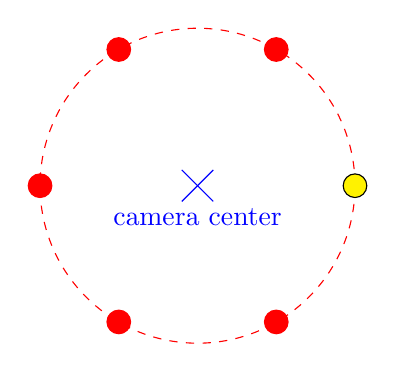
\begin{tikzpicture}
        \draw[red, dashed] (0,0) circle (2);
        \draw[blue] (-0.2,0.2) -- (0.2,-0.2);
        \draw[blue] (0.2,0.2) -- (-0.2,-0.2);
        \draw[blue] (0,-0.4) node {camera center};
        \draw[fill=yellow] (2,0) circle (0.15);
        \draw[red, fill=red] (1,1.73) circle (0.15);
        \draw[red, fill=red] (-1,1.73) circle (0.15);
        \draw[red, fill=red] (-2,0) circle (0.15);
        \draw[red, fill=red] (-1,-1.73) circle (0.15);
        \draw[red, fill=red] (1,-1.73) circle (0.15);
    \end{tikzpicture}
    \caption{If a target (yellow dot) gets observed in wobble mode, the background estimation can be done using a arbitrary number of off regions 
        (red dots) along a circle around the camera center.
    }
    \label{fig:wobble}
\end{figure}

